% !TEX root = marvin.tex
\begin{figure*}[t]
  \begin{center}
  \iflatexml
  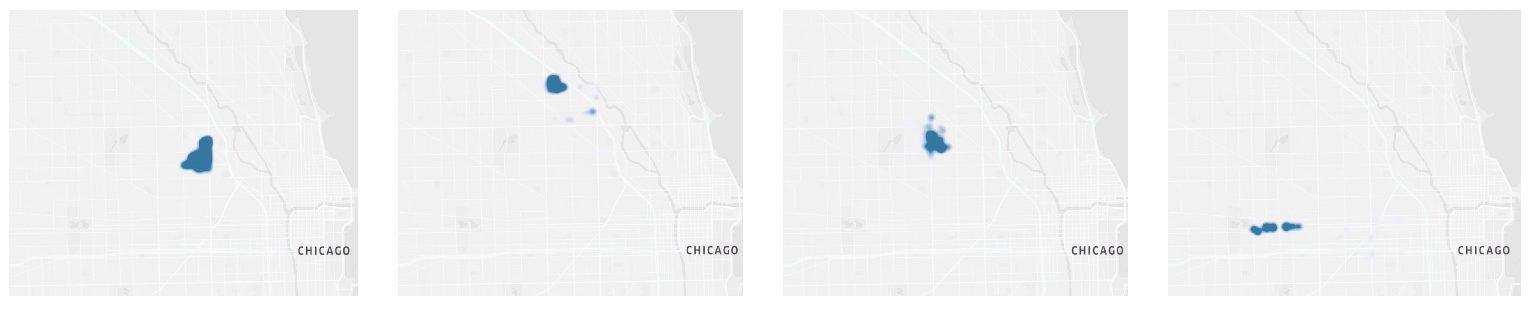
\includegraphics[width=6\textwidth]{figs/heatmap_cluster.png}
  \else
    \begin{tabular}{llll}
      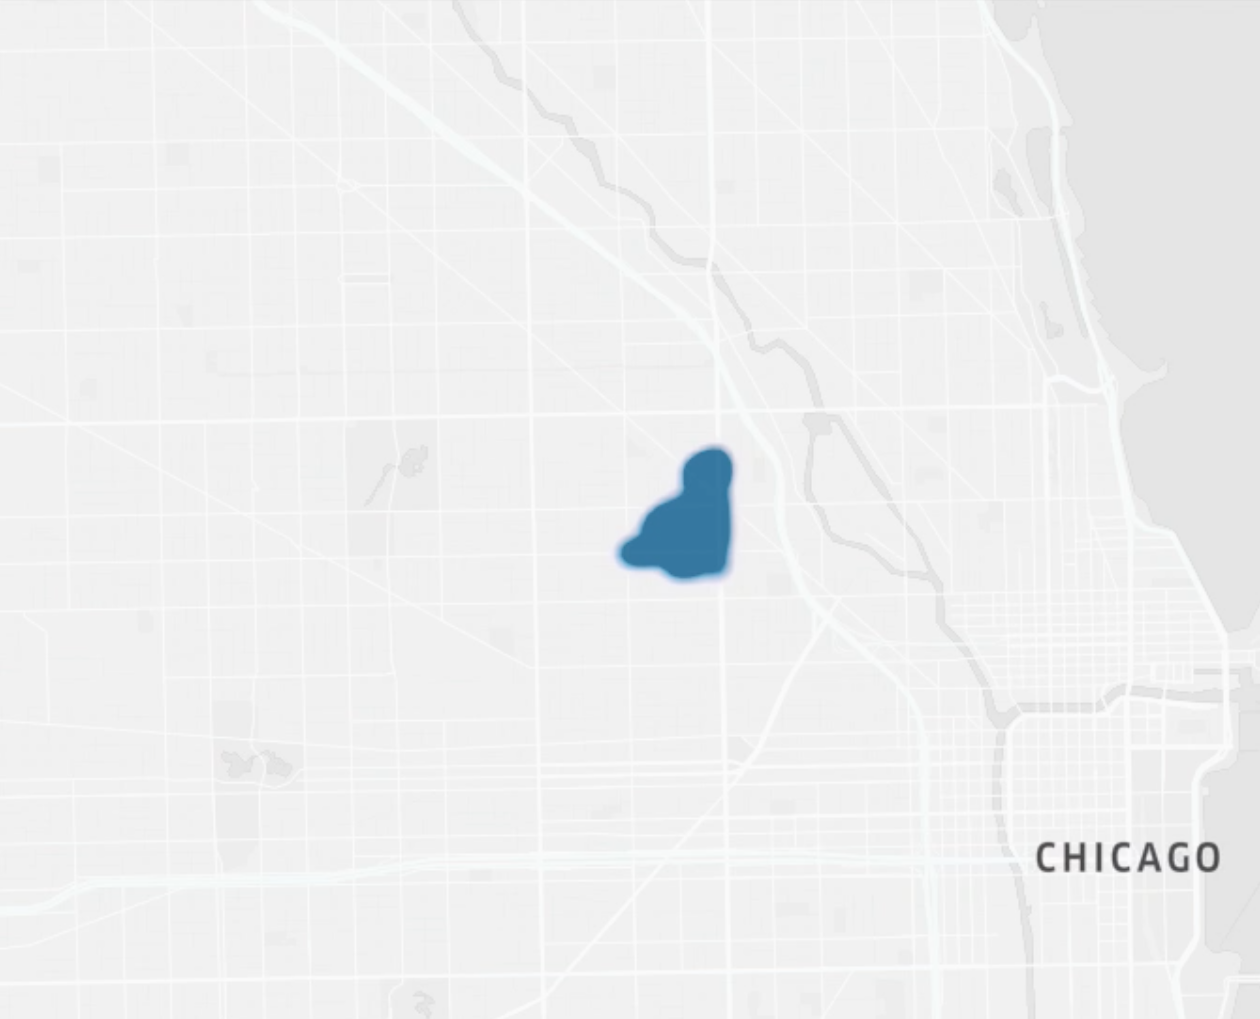
\includegraphics[height=3.0cm,trim={0.2cm 0 0.4cm 0},clip]{figs/clustered1.png} &
      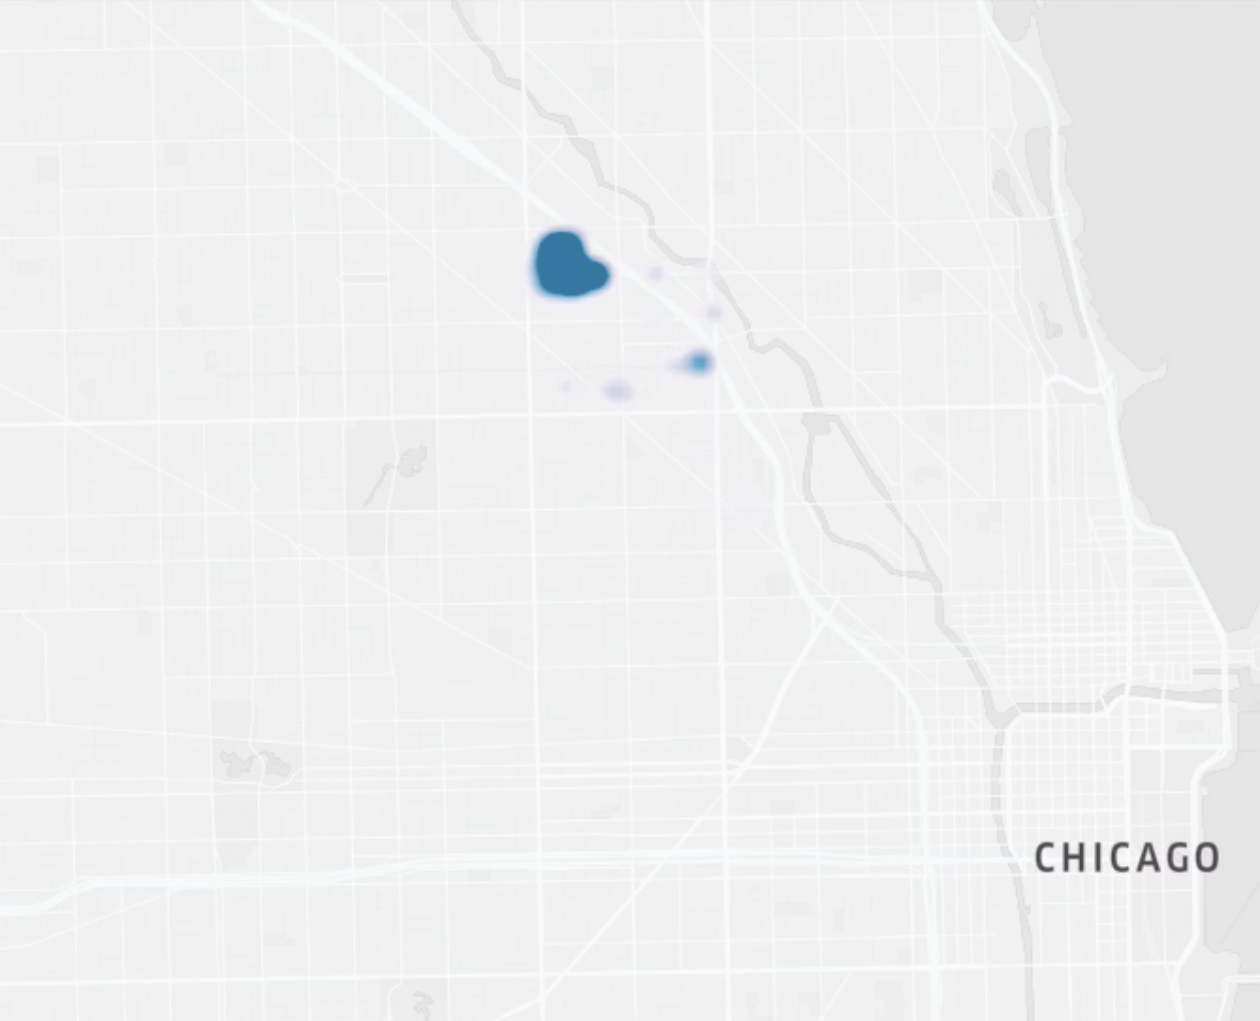
\includegraphics[height=3.0cm,trim={0.2cm 0 0.8cm 0},clip]{figs/clustered2.png} &
      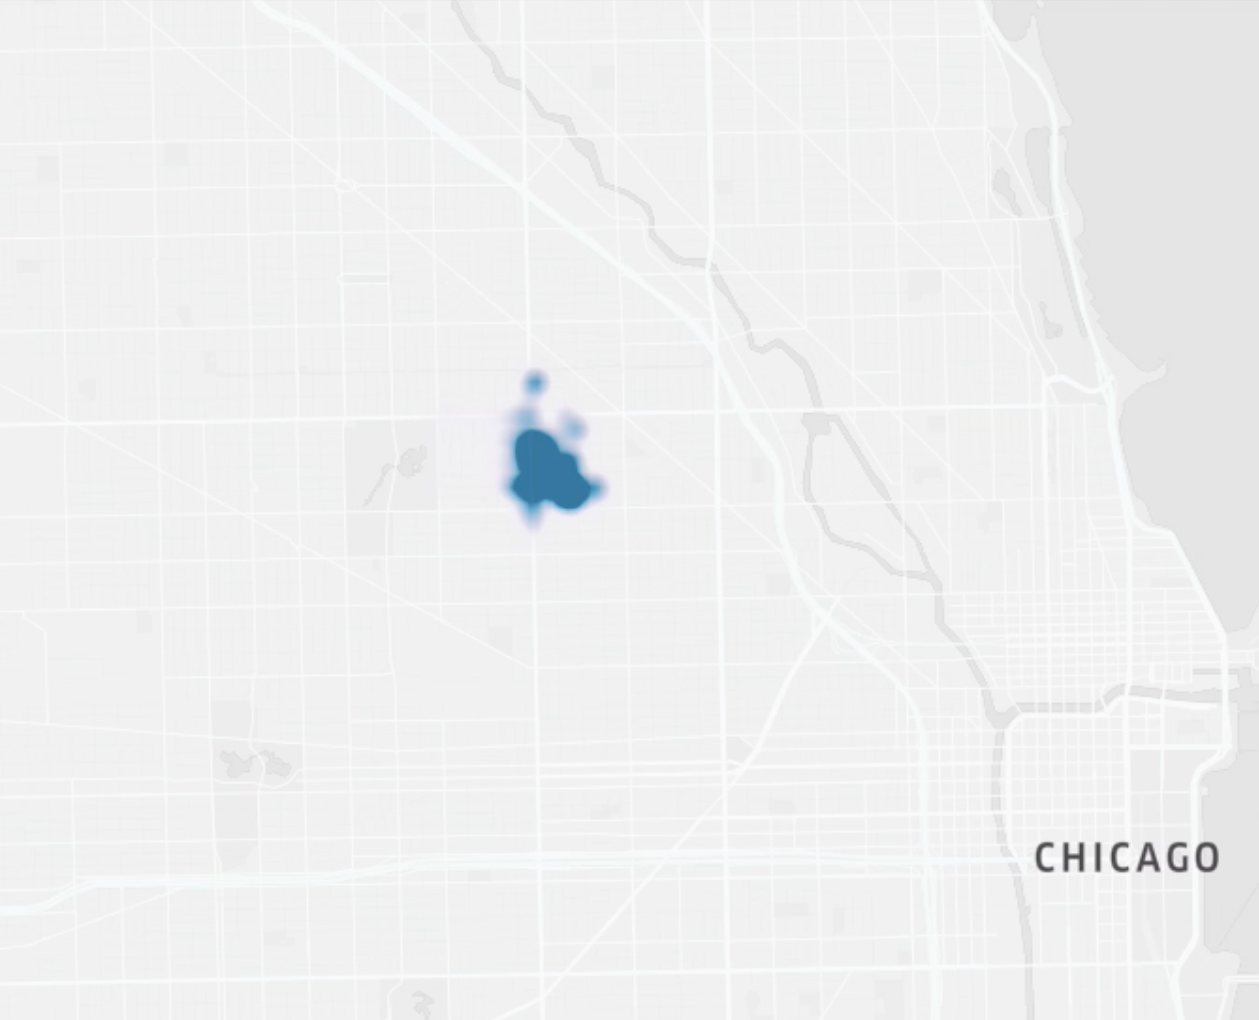
\includegraphics[height=3.0cm,trim={0.2cm 0 0.8cm 0},clip]{figs/clustered3.png} &
      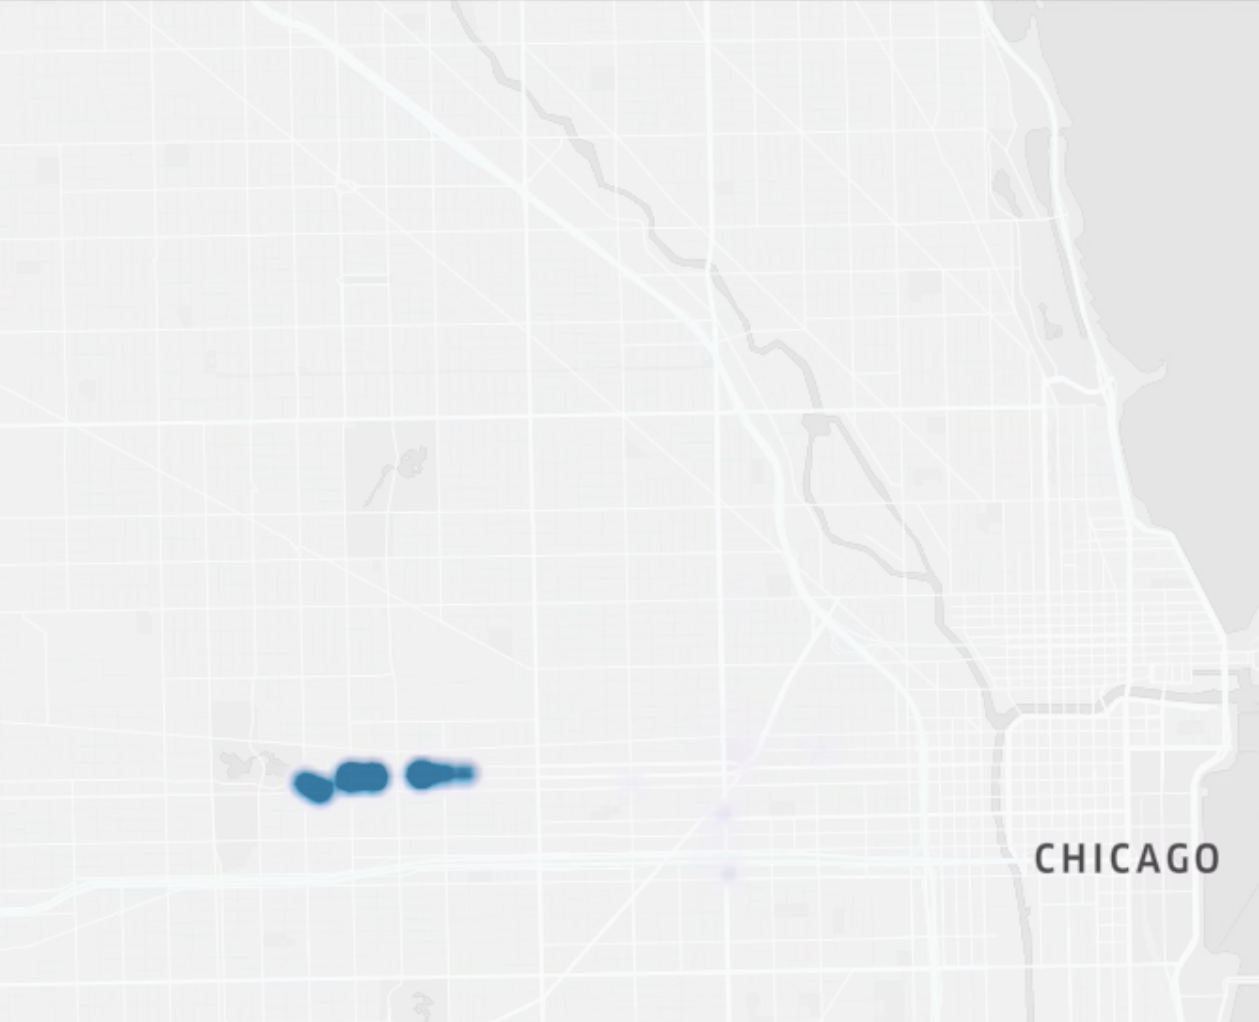
\includegraphics[height=3.0cm,trim={0.0cm 0 0cm 0},clip]{figs/clustered4.png} \\
    \end{tabular}
  \fi
  % \vspace{-0.15in}
  \caption{Value function of an agents while mapping a given region.
  The value function is high around the roads that are close
  to the agent in a sense that implies that this cluster has been
  assigned to that agent. The red dot on the left and the blue dot
  on the right represent the agent's current position.}
  \label{fig:heatmap_cluster}
  \end{center}
  \vspace{-0.25in}
\end{figure*}
